\documentclass[10pt,a4paper]{article}
\usepackage[utf8]{inputenc}
\usepackage[spanish]{babel}
\usepackage{amsmath}
\usepackage{amsfonts}
\usepackage{amssymb}
\usepackage{graphicx}
\usepackage{listings}
\usepackage[left=2cm,right=2cm,top=2cm,bottom=2cm]{geometry}

\begin{document}

\begin{titlepage}
\title{{\Huge Práctica 1 - Seguridad Informática}}
\author{Pedro Tamargo \and Juan José Tambo}
\date{\today}
\clearpage\maketitle
\thispagestyle{empty}
\tableofcontents
\end{titlepage}

\section{Tarea 1: Experimentar con las funciones en Bash}

Para esta sección se ha creado una función \texttt{foo} con código extra y se ha ejecutado el siguiente código:\\

\lstinputlisting{listings/ataque_shell.sh}

Tras la ejecución de este código podemos observar como el intérprete \emph{BASH\_{}SHELLSHOCK} es vulnerable (Figura \ref{fig:tarea1_shellshock}) ya que ha ejecutado el código extra de la función \texttt{foo}.

\begin{figure}[h!]
\centering
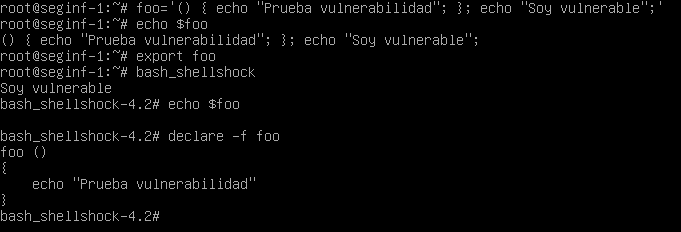
\includegraphics[scale=0.6]{images/Tarea_1.png}
\caption{Intérprete afectado por el ataque \emph{shellshock}}
\label{fig:tarea1_shellshock} 
\end{figure}

Si repetimos el experimento utilizando el intérprete \emph{Bash} con la vulnerabilidad arreglada, se puede observar que al utilizar el código anterior no produce el mismo resultado que en el primer experimento (Figura \ref{fig:tarea1_bash_normal}).

\begin{figure}[h!]
\centering
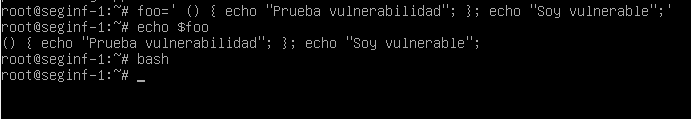
\includegraphics[scale=0.6]{images/Tarea_1b.png}
\caption{Intérprete \textbf{NO} afectado por el ataque \emph{shellshock}}
\label{fig:tarea1_bash_normal} 
\end{figure}

\section{Tarea 2: Configuración de programas CGI}

Hola

\section{Tarea 3: pasar datos a Bash a través de las variables de entorno}

Para enviar un \emph{string} arbitrario al programa \emph{CGI} se ha utilizado el siguiente script:\\

\lstinputlisting{listings/tarea3.cgi}


\section{Tarea 4: Lanzamiento del Ataque Shellshock}

Hola

\section{Tarea 5: Obtención de un Shell inverso a través de un ataque Shellshock}

Hola



\end{document}